\chapter{Methodology and Design Approach}
\label{ch:methodology_design}

\section{Architectural Overview: 5-Tier Modular Monolith}
\label{sec:arch_overview}
To deliver high performance, maintainability, and strict security without the distributed overhead of microservices, CivicSphere AI is architected as a \textbf{5-Tier Modular Monolith}. The architectural blueprint is depicted in Figure~\ref{fig:system_architecture}.

\begin{figure}[H]
\centering
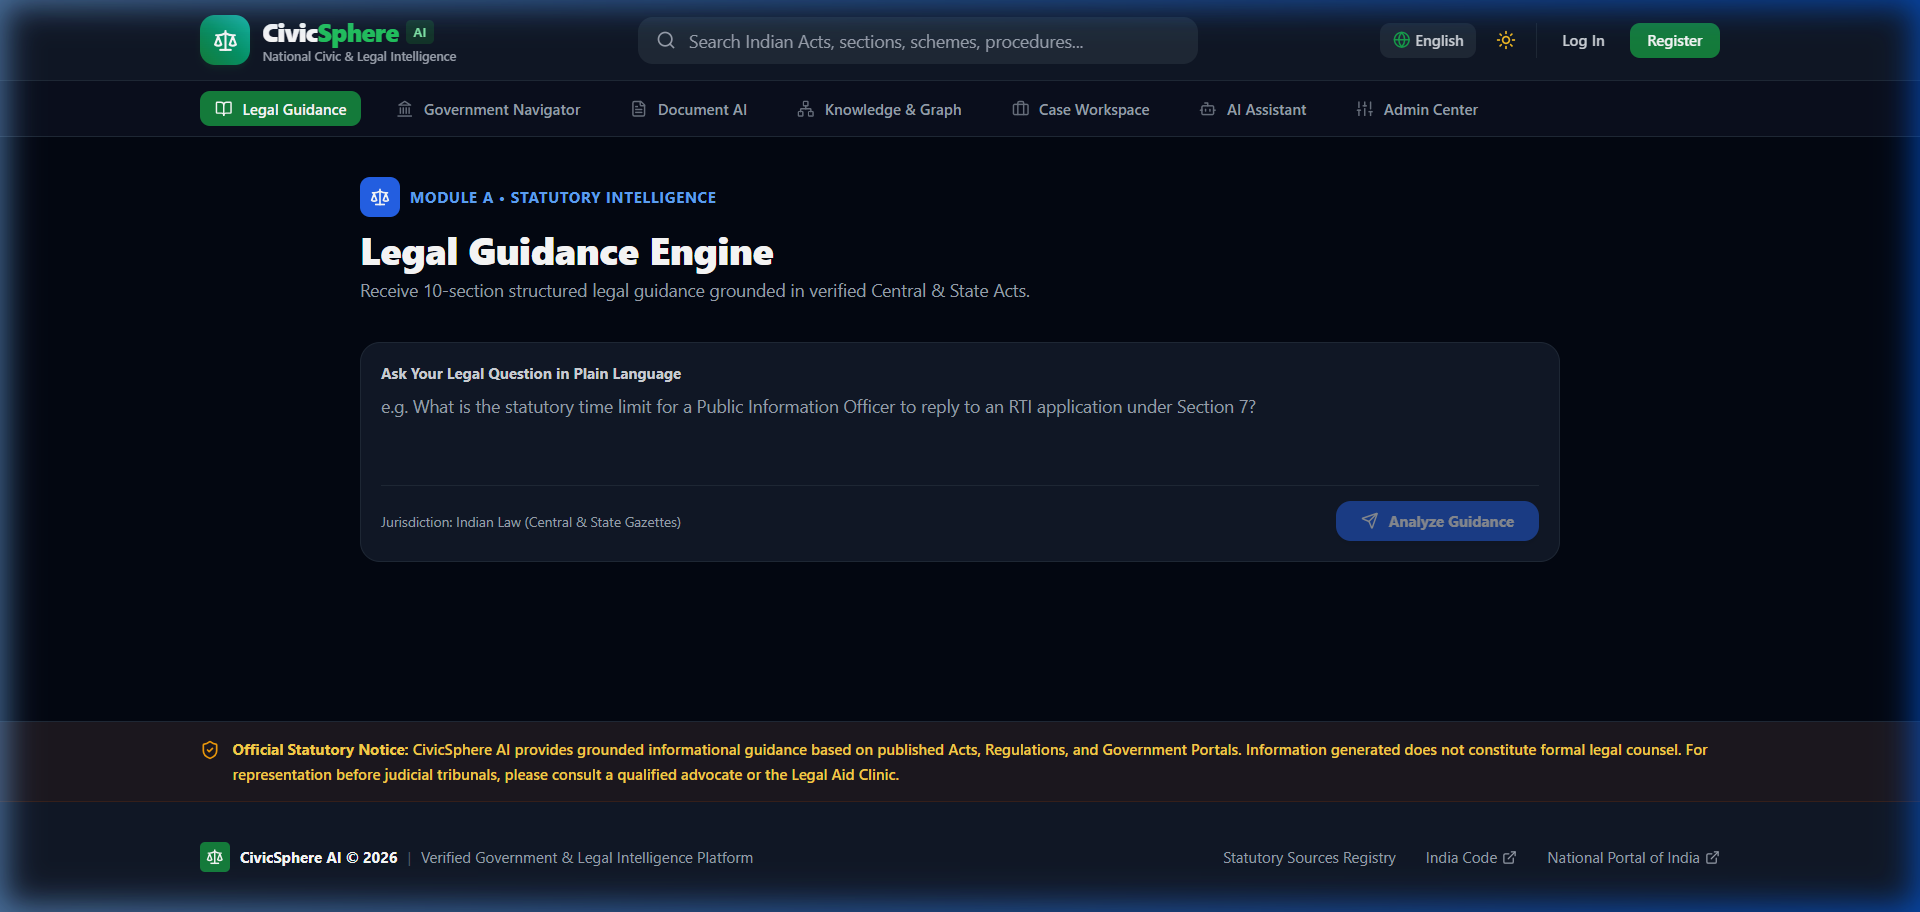
\includegraphics[width=0.9\textwidth]{images/legal_page_view.png}
\caption{System Architecture Blueprint: 5-Tier Modular Monolith of CivicSphere AI.}
\label{fig:system_architecture}
\end{figure}

The five architectural tiers operate as follows:
\begin{enumerate}
    \item \textbf{Tier 1: Presentation Layer (Next.js 16 App Router):} Engineered using React 19, Tailwind CSS, Lucide Icons, and Next.js App Router. Provides a responsive, accessible citizen portal featuring light/dark mode, client-side input sanitization, and 31 statically prerendered routes.
    \item \textbf{Tier 2: API Gateway and Security Perimeter (FastAPI):} Asynchronous ASGI engine managing routing, CORS policies, rate limiting, and dependency-injected JWT authentication with Role-Based Access Control (RBAC).
    \item \textbf{Tier 3: Core Orchestrator and Specialist Agents:} Manages the execution lifecycle across four specialized agents: Legal Guidance Agent, Government Scheme Navigator Agent, Knowledge Graph Agent, and Document Processing Agent.
    \item \textbf{Tier 4: Hybrid Retrieval and Validation Engine:} Implements BM25 lexical search, dense cosine vector embeddings, NetworkX multi-hop graph traversal, and the Gate 2 citation circuit breaker.
    \item \textbf{Tier 5: Persistence and Durable Cloud Storage Layer:} Relational Supabase PostgreSQL for user accounts, case records, and audit logs; private S3-compatible Supabase Object Storage for uploaded citizen documents.
\end{enumerate}

\section{Detailed Module Workflows}
\label{sec:module_workflows}

\subsection{Module A: Legal Guidance Engine}
The Legal Guidance Engine executes when a citizen submits a query regarding a legal right, police conduct, dispute, or notice.
\begin{enumerate}
    \item \textbf{Query Normalization:} Cleans input text, removes noise, and extracts key entities and statutory keywords.
    \item \textbf{Statutory Retrieval:} Executes parallel searches across the indexed 8-Act database using BM25 and vector embeddings.
    \item \textbf{Evidence Assembly:} Compiles retrieved statutory chunks into an immutable \texttt{EvidencePack}.
    \item \textbf{Gate 2 Grounding Evaluation:} Evaluates semantic overlap between retrieved sections and query intent. If overlap ratio $\ge 0.75$, generates grounded guidance; if $< 0.75$, switches to deterministic factual fallback.
    \item \textbf{Action Formatting:} Appends applicable court forums, limitation deadlines, and official e-filing portal URLs.
\end{enumerate}

\subsection{Module B: Government Service Navigator}
The Government Service Navigator assists citizens in identifying and accessing public welfare entitlements.
\begin{enumerate}
    \item \textbf{Profile Ingestion:} Captures applicant parameters (age, annual income, caste/social category, landholding, residency).
    \item \textbf{Rule Evaluation Engine:} Executes deterministic condition evaluation against the 12 seeded scheme definitions.
    \item \textbf{Entitlement Discovery:} Filters matching schemes and highlights qualifying benefits.
    \item \textbf{Document Checklist Compilation:} Outlines mandatory documents (e.g., Aadhaar card, income certificate, bank passbook).
    \item \textbf{Grievance Redressal Linking:} Provides direct deep-links to CPGRAMS and relevant appellate authorities.
\end{enumerate}

\subsection{Module C: Civic Knowledge and Agentic Graph}
Module C provides the relational glue connecting statutory law to administrative welfare schemes.
\begin{enumerate}
    \item \textbf{Graph Modeling:} Maintained in-memory using NetworkX directed multigraphs with 40+ nodes.
    \item \textbf{Multi-Hop Relational Traversal:} When a query relates to an issue spanning multiple domains (e.g., domestic violence requiring police intervention and welfare shelter support), the graph traverses across relational edges (\texttt{governed\_by}, \texttt{escalates\_to}, \texttt{qualifies\_for}).
    \item \textbf{Temporal Freshness Verification:} Nodes include timestamp metadata ensuring amended or repealed acts (IPC) redirect to modern statutes (BNS 2023).
\end{enumerate}

\subsection{Module D: Intelligent Document Processing}
Module D ingests, validates, parses, and persists citizen documents.
\begin{enumerate}
    \item \textbf{Multipart Upload Validation:} Enforces a strict 10MB file limit and MIME validation (\texttt{application/pdf}).
    \item \textbf{Durable Cloud Storage:} Asynchronously streams file bytes to a private Supabase S3 bucket (\texttt{civicsphere-documents}) and generates a signed, time-limited retrieval token.
    \item \textbf{Heuristic Text and Entity Parsing:} Utilizes pdfplumber with PyPDF fallback to extract text, followed by regular expression pattern matchers extracting notice dates, case numbers, statutory sections, and penalty demands.
    \item \textbf{Classification:} Classifies documents into Court Summons, Legal Notice, Violation Challan, or Scheme Form within $< 2.0$ seconds.
\end{enumerate}

\section{14-Step End-to-End Processing Workflow}
\label{sec:14step_workflow}
The end-to-end execution of a citizen interaction is formalized across 14 discrete, deterministic steps:
\begin{itemize}
    \item \textbf{Step 1 (Citizen Query Input):} User submits text or document via the web portal.
    \item \textbf{Step 2 (Client Validation):} Next.js validates input length, sanitizes strings, and checks file MIME headers.
    \item \textbf{Step 3 (Gateway Ingestion):} FastAPI verifies JWT bearer token (if authenticated) and applies rate limits.
    \item \textbf{Step 4 (Intent Classification):} Routes query to Legal, Scheme, Document, or General Orchestrator.
    \item \textbf{Step 5 (Agent Dispatch):} Instantiates domain specialist agent with isolated execution context.
    \item \textbf{Step 6 (Hybrid Lexical/Vector Search):} Executes parallel BM25 and dense vector retrieval.
    \item \textbf{Step 7 (Knowledge Graph Multi-Hop Search):} Interrogates NetworkX graph for relational cross-links.
    \item \textbf{Step 8 (Evidence Pack Assembly):} Ranks and merges Top-5 statutory and scheme chunks into an immutable payload.
    \item \textbf{Step 9 (Gate 2 Verification Circuit):} Validates citation grounding and checks claim-to-evidence ratio.
    \item \textbf{Step 10 (Response Synthesis):} Generates plain-language guidance with verifiable inline citations.
    \item \textbf{Step 11 (Safety and Disclaimer Injection):} Injects statutory legal disclaimers and legal-aid helpline numbers.
    \item \textbf{Step 12 (Audit Logging):} Writes non-identifiable query metadata and performance timestamps to database.
    \item \textbf{Step 13 (UI Rendering):} Returns JSON payload; Next.js renders guidance with interactive citation cards.
    \item \textbf{Step 14 (Case Dossier Archival):} User optionally saves guidance and attached documents to personal workspace.
\end{itemize}

\section{Evidence-Grounded Synthesis and Gate 2 Circuit Breaker}
\label{sec:gate2_circuit_breaker}
The mathematical formulation of the Gate 2 circuit breaker is defined as:
\begin{equation}
\Gamma(Q, \mathcal{E}) = 
\begin{cases} 
\text{NeuralSynthesis}(Q, \mathcal{E}) & \text{if } \text{Sim}(Q, \mathcal{E}) \ge \tau \land \text{Citations}(\mathcal{E}) \neq \emptyset \\
\text{DeterministicFallback}(Q, \mathcal{E}_{fallback}) & \text{otherwise}
\end{cases}
\label{eq:gate2_logic}
\end{equation}
where $\tau = 0.75$ is the empirical confidence threshold. This guarantees that ungrounded queries never produce fabricated advice.
